\documentclass[fleqn]{article}

%% Created with wxMaxima 23.12.0

\setlength{\parskip}{\medskipamount}
\setlength{\parindent}{0pt}
\usepackage{iftex}
\ifPDFTeX
  % PDFLaTeX or LaTeX 
  \usepackage[utf8]{inputenc}
  \usepackage[T1]{fontenc}
  \DeclareUnicodeCharacter{00B5}{\ensuremath{\mu}}
\else
  %  XeLaTeX or LuaLaTeX
  \usepackage{fontspec}
\fi
\usepackage{graphicx}
\usepackage{color}
\usepackage{amsmath}
\usepackage{grffile}
\usepackage{ifthen}
\newsavebox{\picturebox}
\newlength{\pictureboxwidth}
\newlength{\pictureboxheight}
\newcommand{\includeimage}[1]{
    \savebox{\picturebox}{\includegraphics{#1}}
    \settoheight{\pictureboxheight}{\usebox{\picturebox}}
    \settowidth{\pictureboxwidth}{\usebox{\picturebox}}
    \ifthenelse{\lengthtest{\pictureboxwidth > .95\linewidth}}
    {
        \includegraphics[width=.95\linewidth,height=.80\textheight,keepaspectratio]{#1}
    }
    {
        \ifthenelse{\lengthtest{\pictureboxheight>.80\textheight}}
        {
            \includegraphics[width=.95\linewidth,height=.80\textheight,keepaspectratio]{#1}
            
        }
        {
            \includegraphics{#1}
        }
    }
}
\newlength{\thislabelwidth}
\DeclareMathOperator{\abs}{abs}

\definecolor{labelcolor}{RGB}{100,0,0}

\begin{document}


\noindent
%%%%%%%%
%% INPUT:
\begin{minipage}[t]{4.000000em}\color{red}\bfseries
(\% i1)	
\end{minipage}
\begin{minipage}[t]{\textwidth}\color{blue}
kill(all)\$
\end{minipage}

\noindent%



\noindent
%%%%%%%%
%% INPUT:
\begin{minipage}[t]{4.000000em}\color{red}\bfseries
 --\ensuremath{\ensuremath{>}}	
\end{minipage}
\begin{minipage}[t]{\textwidth}\color{blue}
/*\ see\ README\_moss\ */\\
/*\ plot\ against\ normalized\ reference\ */
\end{minipage}

\noindent%



\noindent
%%%%%%%%
%% INPUT:
\begin{minipage}[t]{4.000000em}\color{red}\bfseries
(\% i4)	
\end{minipage}
\begin{minipage}[t]{\textwidth}\color{blue}
Uo:1\$\ /*\ applied\ voltage\ */\\
R:2\$\ \ /*\ resistance\ */\\
C:0.2\$\ \ /*\ capacity\ by\ experiment\ */\\
tau:\ 1\$
\end{minipage}

\noindent%



\noindent
%%%%%%%%
%% INPUT:
\begin{minipage}[t]{4.000000em}\color{red}\bfseries
(\% i6)	
\end{minipage}
\begin{minipage}[t]{\textwidth}\color{blue}
chargeUc(t):=Uo*(1-exp(-t/R/C));\\
refchargeUc(t):=1*(1-exp(-t/1/1));
\end{minipage}
%%%% OUTPUT:
\[\displaystyle \tag{\% o5} 
\mathop{chargeUc}(t)\mathop{:=}\ensuremath{\mathrm{Uo}}\, \left( 1\mathop{-}\mathop{exp}\left( \frac{\frac{\mathop{-}t}{R}}{C}\right) \right) \mbox{}\]

\[\tag{\% o6} 
\mathop{refchargeUc}(t)\mathop{:=}1 \left( 1\mathop{-}\mathop{exp}\left( \frac{\frac{\mathop{-}t}{1}}{1}\right) \right) \mbox{}
\]
%%%%%%%%%%%%%%%%


\noindent
%%%%%%%%
%% INPUT:
\begin{minipage}[t]{4.000000em}\color{red}\bfseries
(\% i8)	
\end{minipage}
\begin{minipage}[t]{\textwidth}\color{blue}
disUc(t):=Uo*exp(-t/R/C);\\
refdisUc(t):=1*exp(-t/1/1);
\end{minipage}
%%%% OUTPUT:
\[\displaystyle \tag{\% o7} 
\mathop{disUc}(t)\mathop{:=}\ensuremath{\mathrm{Uo}} \mathop{exp}\left( \frac{\frac{\mathop{-}t}{R}}{C}\right) \mbox{}\]

\[\tag{\% o8} 
\mathop{refdisUc}(t)\mathop{:=}1 \mathop{exp}\left( \frac{\frac{\mathop{-}t}{1}}{1}\right) \mbox{}
\]
%%%%%%%%%%%%%%%%


\noindent
%%%%%%%%
%% INPUT:
\begin{minipage}[t]{4.000000em}\color{red}\bfseries
(\% i9)	
\end{minipage}
\begin{minipage}[t]{\textwidth}\color{blue}
wxplot2d([chargeUc(t),disUc(t),refchargeUc(t),refdisUc(t)],\ [t,\ 0.,\ 5*tau],grid2d\ )\$
\end{minipage}
%%%% OUTPUT:
\[\displaystyle \tag{\% t9} 
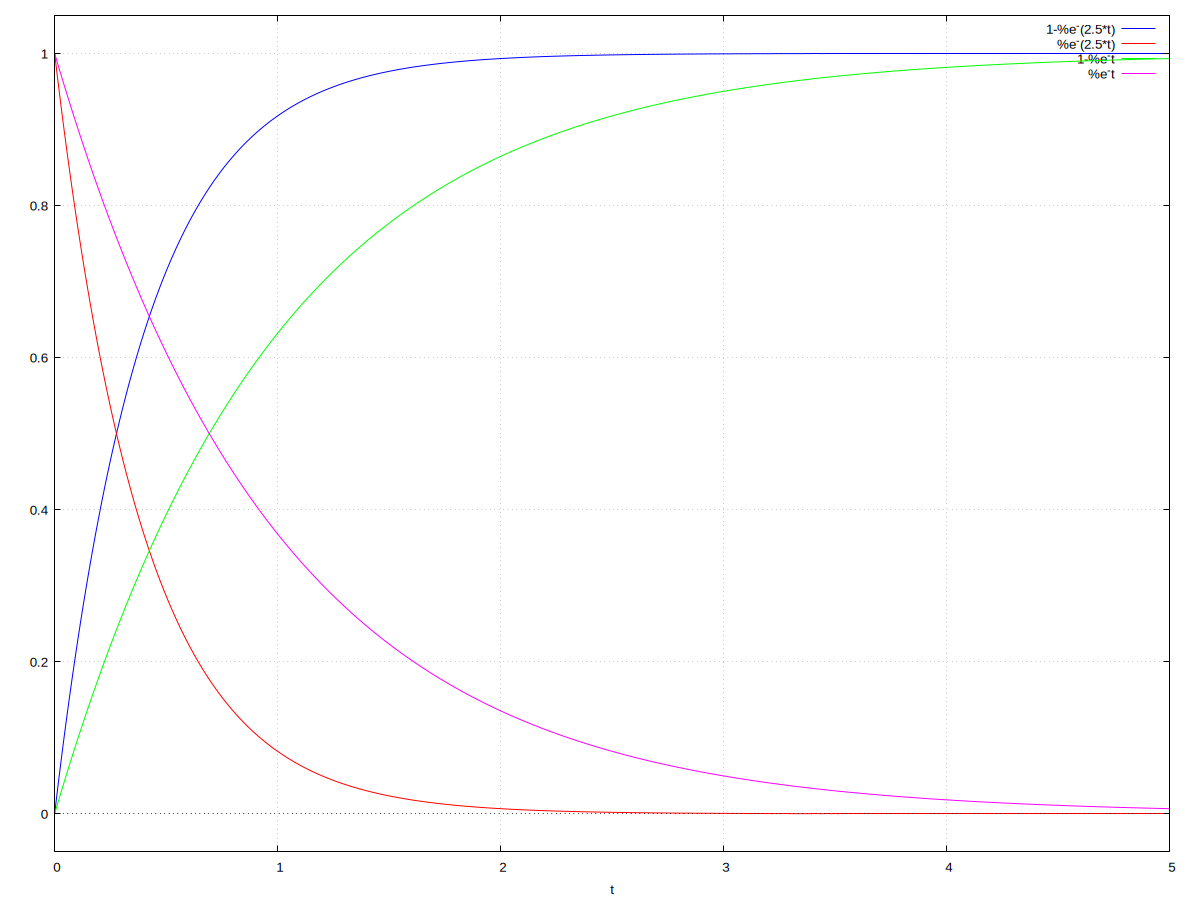
\includegraphics[width=.95\linewidth,height=.80\textheight,keepaspectratio]{capacitor-plot_v1_img/capacitor-plot_v1_1}\mbox{}
\]
%%%%%%%%%%%%%%%%


\noindent
%%%%%%%%
%% INPUT:
\begin{minipage}[t]{4.000000em}\color{red}\bfseries
 --\ensuremath{\ensuremath{>}}	
\end{minipage}
\begin{minipage}[t]{\textwidth}\color{blue}
/*\ eqnL:\ 0.98\ =\ Uo*(1-exp(-5/R/C))\$\ /*\ charge\ */\\
eqnD:\ 0.90\ =\ Uo*exp(-2.5/R/C)\$\ /*\ discharge\ */
\end{minipage}

\noindent%



\noindent
%%%%%%%%
%% INPUT:
\begin{minipage}[t]{4.000000em}\color{red}\bfseries
 --\ensuremath{\ensuremath{>}}	
\end{minipage}
\begin{minipage}[t]{\textwidth}\color{blue}
/*\ solL:\ rhs(solve(eqnL,R)[5]);\\
solD:\ rhs(solve(eqnD,R)[5]);\\
solve([eqn1,eqn2],R);\\
solve(sol1=sol2,C);\ 
\end{minipage}

\noindent%

\end{document}
